\documentclass[a4paper,12pt]{article}

\usepackage[russian]{babel}
\usepackage{cmap}
\usepackage[utf8]{inputenc}
\usepackage[usenames]{color}
\usepackage{tabularray}
\usepackage{xcolor}
\usepackage{graphicx} 
\usepackage{subfigure}
\usepackage{subcaption}

\usepackage[unicode]{hyperref} % цвета гиперссылок
\hypersetup{
	colorlinks,
	citecolor=black,
	filecolor=black,
	linkcolor=blue,
	urlcolor=black
}

\usepackage{geometry} % задаёт поля 
%\geometry{left=3cm}
%\geometry{right= 1.5cm}
%\geometry{top=2cm}
%\geometry{bottom=2cm} 

\usepackage{enumitem} % настраивает работу со списками:
\def\labelitemi{—} % ... задаёт длинное тире как стандартный маркер ненумерованного списка
\setlist{nolistsep} %  ... убирает дополнительный отступы между элементами списка


% удаляет названия и продолжение следует и т. для таблиц, будет только таблица без всего
\DefTblrTemplate{contfoot-text}{default}{}
\DefTblrTemplate{conthead-text}{default}{}
\DefTblrTemplate{caption}{default}{}
\DefTblrTemplate{conthead}{default}{}
\DefTblrTemplate{capcont}{default}{}


\title{Поиск калибровочных границ методами машинного обучения}
\author{В. Г. Мосин}
\date{}

%   \input{preamble.tex}
\begin{document}
	\maketitle
	\abstract{\noindent  Предложен метод, позволяющий по данной дискретной случайной величине вычислять границы отклонений, превышение которых дает аномальное значение. Проведена серия компьютерных экспериментов, благодаря которым сформулированы и указаны границы применения метода. Рассмотрены примеры на синтетических данных.}
	
\tableofcontents
	
\section{Введение}
Метод калибровки в анализе качества промышленных изделий представляет собой процесс сравнения измеряемых значений с известными стандартами или эталонами для определения точности и достоверности измерений. Этот метод позволяет проверять соответствие изделий установленным стандартам качества и выявлять любые отклонения от них. Отклонение измеряемых значений от эталонного значения, превышающее некоторую заранее известную величину, означает аномалию, которую следует локализовать и устранить. Метод калибровки хорошо работает в промышленном производстве, когда характеристики изделий — размеры, допуски и т. д. — известны заранее. 
Однако есть целый ряд ситуаций, когда они неизвестны. Например, при изучении биржевых показателей у ценной бумаги нет эталонной цены: сегодня ее цена такова, а завтра она взлетит, или, наоборот, рухнет. И отклонение цены (выражаясь бухгалтерским языком, волатильность ценной бумаги), которое можно считать нормальным, тоже неизвестно: в одни периоды цены стабильны, а в другие — подвержены высоким колебаниям.


\subsection{Теоретическая часть}


Любой измеряемый показатель является дискретной случайной величиной, подверженной небольшому нормальному шуму. Мы будем называть калибровочным значением измеряемого показателя его среднее значение за период измерений (в другой период это может быть другое значение), а калибровочной границей мы будем называть величину отклонения случайной величины от калибровочного значения, превышение которой означает аномалию.
Если известны как калибровочное значение, так и калибровочная граница, то определение нормы или аномалии — это детская задача: измеряем величину, вычисляем разность между полученным значением и эталонным, и если по абсолютной величине она меньше калибровочной границы, то это норма, а если больше — то аномалия.
Нас будет интересовать ситуация, когда калибровочная граница неизвестна.




\subsection{Постановки задачи}

\subsubsection{Предмет исследования}

Предметом нашего исследования будет новый алгоритм поиска калибровочных значений, основанный на вычислении так называемой локтевой точки, которая позволяет отделить величины с большими отклонениями от величин с малыми отклонениями от нормы. Функция поиска локтевой точки так же является авторской, она построена на принципе линеаризации целевой переменной (см. [5]) и успешно применяется нами для решения различных задач.

\subsubsection{Методика исследования} 

Мы генерируем множественные синтетические данные, про которые нам заранее известны все характеристики их анормальности: выраженность аномальных значений и их доля в общем числе наблюдений. Прогоняя синтетические данные через наш алгоритм, мы получаем аномалии, выявленные алгоритмом вслепую, и сравниваем результат с априорно известными нам аномалиями. Условия, при которых результаты близки или совпадают, указывают на условия, в которых наш алгоритм может быть применим.

\subsubsection{Цель исследования} 

Реализовать алгоритм поиска калибровочной границы и указать условия его применения.

\subsection{Технологии}

\subsubsection{Стандартные библиотеки}

Для выполнения вычислений и анализа данных мы пользуемся средой \texttt{Jupyter Notebook}, которая предоставляет удобные средства для работы с языком программирования Python и его главными библиотеками: \texttt{NumPy}, \texttt{Pandas}, \texttt{sklearn} и \texttt{matplotlib}. Благодаря этим инструментам, мы можем эффективно работать с данными, выполнять исследования и визуализировать результаты (см. [1], [2]). 



%Библиотека \texttt{numpy} является одной из ключевых библиотек для научных вычислений и обработки массивов данных в языке программирования \texttt{Python}. Библиотека \texttt{pandas}~--- одна из наиболее популярных и мощных библиотек для работы с данными в языке программирования \texttt{Python} (см. [1]). 
%
%Библиотека \texttt{scikit-learn}, широко известная как \texttt{sklearn}, предоставляет обширный набор инструментов и функций для решения различных задач в языке программирования Python, таких как задачи классификации, регрессии, кластеризации и др. Мы используем эту библиотеку для решения регрессионных задач.

\subsubsection{Авторские функции}

Мы используем функцию поиска локтевой точки \texttt{fold\_point}, которая принимает в качестве аргументов два одномерных массива A и B одинаковой длины, причем, массив A выступает в качестве горизонтальной переменной некоторой заданной таблично функции, а массив B — в качестве вертикальной. Функция исполняет алгоритм линеаризации (cм. [5]) функции B с разбиением на два участка и построением регрессионной сплит-модели, оптимизируя разбиение по максимуму коэффициента детерминации. Функция \texttt{fold\_point(A, B)} возвращает номер \texttt{fold\_num} массива \texttt{A}, в котором достигается максимум, а точка с координатами \texttt{(A(fold\_num), B(fold\_num))} — это и есть искомая точка максимума.


\section{Генератор синтетических данных}


\subsection{Константы и параметры генерации}


Задаем необходимые константы: 

\medskip\noindent
\begin{enumerate}
	\item \texttt{N} — объем выборки,
	\item \texttt{noise\_mean} — среднее значение естественных отклонений, возникающих при измерении показателя, 
	\item \texttt{noise\_std} — среднее квадратичное отклонение естественных отклонений,
\end{enumerate}


\medskip\noindent
и параметры генерации синтетических аномалий:

\medskip\noindent
\begin{enumerate}
	\item \texttt{out\_coef} — коэффициент, при помощи которого мы будем варьировать выраженность аномалий,
	\item \texttt{out\_pro} — процент аномальных значений в выборке объема \texttt{N}.
\end{enumerate}

\subsection{Случайный шум}

Для генерации синтетического показателя \texttt{y}, имитирующего результаты измерений какого-либо реального показателя, воспользуемся методом \texttt{normal} из модуля \texttt{random} библиотеки \texttt{numpy}, который генерирует набор чисел, распределенных по нормальному закону:
\begin{verbatim}
y = np.random.normal(noise_mean, noise_std, N)
\end{verbatim}

\subsection{Аномальные отклонения и их позиции}

Мы будем варьировать две величины: выраженность аномалии, то есть то, насколько аномальное значение отстоит от нормальных значений, и процент аномалий в общей выборке. Выраженность аномалии получается при помощи коэффициента, на который умножается естественный шум: если коэффициент нулевой, то сдвига не происходит вообще, если двукратный — то выраженность аномалии весьма слаба, если десятикратный — выраженность высокая. Для этого вводим переменную \texttt{out\_shift}:

\begin{verbatim}
out_shift = noise_std*out_coef
\end{verbatim}

Далее, выполняем случайную выборку из набора номеров показателя \texttt{y} так, чтобы объем этой выборки составлял нужный нам процент \texttt{k} от объема \texttt{N}. Для этого нужно выбрать 

\begin{verbatim}
k = N*(out_pro/100)
\end{verbatim}
элементов, но проблема в том, что процент аномалий \texttt{out\_pro} не обязан быть целым, а число \texttt{N} не обязано делиться на 100. Другими словами, выражение в правой части относится к типу \texttt{float}, что противоречит здравому смыслу: мы не можем создавать множество, в котором присутствует дробное число элементов. Поэтому мы переводим полученное значение k в формат \texttt{integer}:

\begin{verbatim}
k = int(k)
\end{verbatim}
Теперь из списка номеров \texttt{list(np.arange(N))} извлекаем случайным образом \texttt{k} номеров при помощи метода \texttt{sample} библиотеки \texttt{random}:

\begin{verbatim}
out_num = random.sample(list(np.arange(N)), k)
\end{verbatim}
Остается на позиции с номерами из \texttt{out\_num} записать величины, смещенные на \texttt{out\_shift}.


\subsection{Внедрение аномалий}

Проводим цикл по всем номерам из \texttt{out\_num} и выполняем на каждом шаге смещение на \texttt{out\_shift}:

\begin{verbatim}
for i in out_num: 
    y[i] = y[i] + out_shift
\end{verbatim}
Теперь в массиве y присутствуют аномальные значения. Их число составляет \texttt{out\_pro} процентов от общего объема, и они смещены относительно своих нормальных положений на  \texttt{out\_shift} (см. рис. 1 и 2).

\subsection{Примеры}

На первом из рисунков в серии рис. 1 мы использовали
\begin{verbatim}
out_pro  = 7
out_coef = 0
\end{verbatim}
Понятно, что при этом \texttt{out\_shift = 0}, и аномалий, которые мы помечали желтыми точками, нет вообще. На втором рисунке мы задали
\begin{verbatim}
out_pro  = 7
out_coef = 3
\end{verbatim}
Теперь отклонение аномалий \texttt{out\_shift} в три раза больше нормального шума \texttt{nise\_std} и, тем не менее, аномалии выражены настолько слабо, что возникает вопрос: а аномалии ли это? На третьем рисунке значения параметров таковы:
\begin{verbatim}
out_pro  = 7
out_coef = 8
\end{verbatim}
то есть, при восьмикратном увеличении отклонений аномалии становятся выраженными.

\begin{figure}[!h]
	\centering
	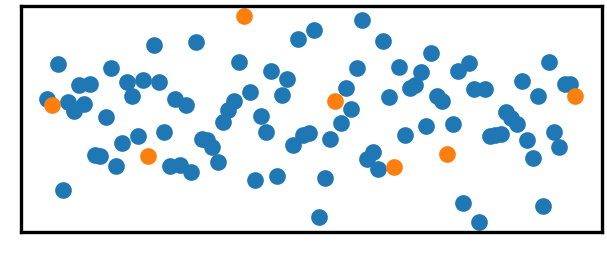
\includegraphics[width=0.25\linewidth]{pictures/Аномалии 0}
	\hspace{0.01\linewidth}
	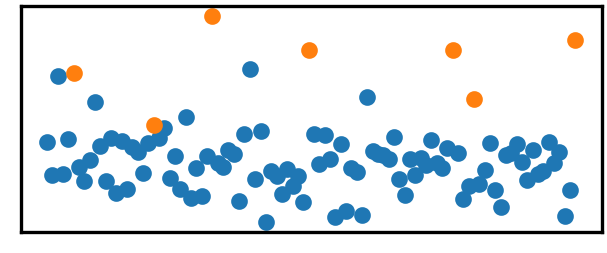
\includegraphics[width=0.25\linewidth]{pictures/Аномалии 3}
	\hspace{0.01\linewidth}
	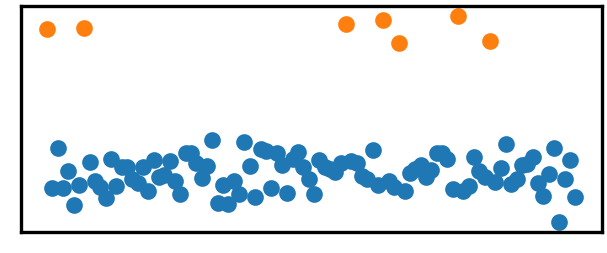
\includegraphics[width=0.25\linewidth]{pictures/Аномалии 8}
	\\
	\caption{Примеры распределения аномалий по выраженности}
\end{figure}

В рисунках серии рис. 2. мы, наоборот, зафиксировали выраженность аномалий и изменяли их процент. На первом рисунке
\begin{verbatim}
out_pro  = 1
out_coef = 8
\end{verbatim}
Поскольку для иллюстрации идеи мы использовали 100 точек, понятно, что мы получили 99 нормальных точек и одну аномальную. На втором рисунке мы увеличили процент аномалий, оставив ту же выраженность
\begin{verbatim}
out_pro  = 10
out_coef = 8
\end{verbatim}
а на третьем — довели процент аномальных точек до 40
\begin{verbatim}
out_pro  = 40
out_coef = 8
\end{verbatim}
в результате чего возник еще один вопрос: являются ли эти точки аномальными, если их так много, и не являются ли они типичными, но относящимися к другому типу?

\begin{figure}[!h]
	\centering
	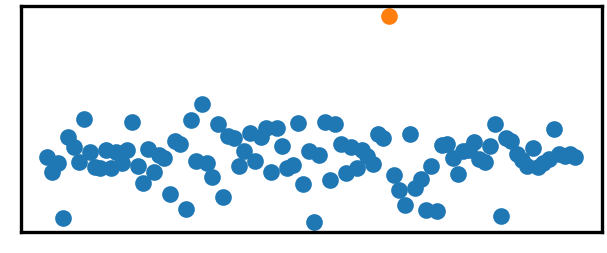
\includegraphics[width=0.25\linewidth]{pictures/Аномалии 1 про}
	\hspace{0.01\linewidth}
	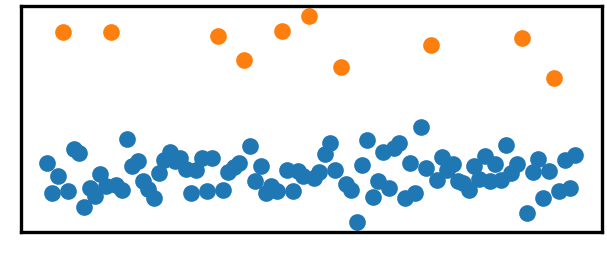
\includegraphics[width=0.25\linewidth]{pictures/Аномалии 10 про}
	\hspace{0.01\linewidth}
	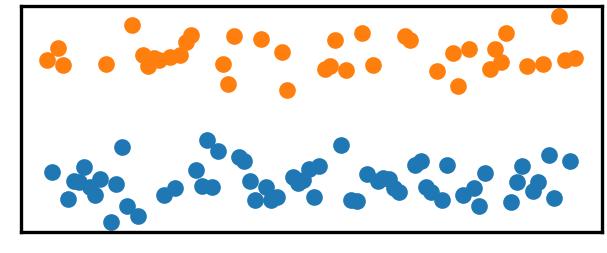
\includegraphics[width=0.25\linewidth]{pictures/Аномалии 40 про}
	\\
	\caption{Примеры распределения аномалий по объему}
\end{figure}

Мы еще вернемся к этим вопросам в разделе 4.

\section{Алгоритм} 

Мы будем варьировать два параметра: \texttt{out\_coef}, который определяет степень выраженности аномалии, и \texttt{out\_pro}, который задает процент аномальных значений, причем коэффициент \texttt{out\_coef} мы будем изменять в цикле в пределах от 1 до 9, а процент \texttt{out\_pro} — от 1\% до 99\% (см. рис. 3 в следующем разделе).


\subsection{Установка стартовых значений цикла и генерация данных}

Устанавливаем значения констант:
\begin{verbatim}
N = 1000
noise_mean = 0 
noise_std= 0.1
\end{verbatim}
и присваиваем параметрам \texttt{out\_pro} и \texttt{out\_coef} стартовые значения:
\begin{verbatim}
out_pro  = 1
out_coef = 1
\end{verbatim}
Затем исполняем шаги 2.2–2.4.  В результате получаем случайную величину  \texttt{y} объема \texttt{N}, которая содержит 1\% выбросов, выраженных с малым коэффициентом выраженности.


\subsection{Вычисление отклонений}


Пользуясь методами  \texttt{mean} и \texttt{abs}, вычисляем массив отклонений случайной величины \texttt{y} от ее среднего значения:
\begin{verbatim}
fluctation = abs(y.mean() - y)
\end{verbatim}

\subsection{Агрегация промежуточных результатов}

Нам понадобится промежуточная система для хранения и обработки вычисляемых величин. Для этого, пользуясь методом \texttt{DataFrame} библиотеки \texttt{pandas}, мы создаем пустой датафрейм, в который будем записывать необходимые для дальнейших действий сведения
\begin{verbatim}
df = pd.DataFrame() 
\end{verbatim}
Помещаем в него случайную величину y и массив \texttt{fluctuation}:
\begin{verbatim}
df['y'] = y
df['fluctation'] = fluctuation
\end{verbatim}

\subsection{Сортировка отклонений}


Пользуясь методом \texttt{sort\_values} библиотеки \texttt{pandas}, упорядочиваем объекты датафрейма \texttt{df} по убыванию величины отклонения и помещаем результат в датафрейм \texttt{df\_sorted}:
\begin{verbatim}
df_sorted = df.sort_values(by='fluctation', ascending=False)
\end{verbatim}


\subsection{Поиск локтевой точки}

На предыдущем шаге мы получили массив упорядоченных по убыванию отклонений, элементы которого нумеруются от 0 до \texttt{N–1}. Следовательно, мы имеем таблично заданную функцию, к которой можно применить алгоритм поиска локтевой точки. Пользуясь методом \texttt{arange} библиотеки \texttt{numpy}, формируем массив горизонтальной переменной:
\begin{verbatim}
A = np.arange(N)
\end{verbatim}
Пользуясь методом \texttt{to\_numpy()} библиотеки \texttt{pandas}, переводим в массив столбец дата-фрейма, к котором записаны абсолютные величины вертикальной переменной:
\begin{verbatim}
B = df_sorted['fluctation'].to_numpy()
\end{verbatim}
Затем применяем к массивам \texttt{A} и \texttt{B} функцию \texttt{fold\_point}, в результате чего получаем номер \texttt{fold\_num}, в котором наблюдается локтевая точка массива отклонений:
\begin{verbatim}
fold_num = fold_point(A, B)
\end{verbatim}


\subsection{Процент обнаруженных аномалий}

Все элементы, которые в массиве B находятся левее номера \texttt{fold\_num}, являются аномалиями, которые обнаружил алгоритм. Поэтому процент обнаруженных аномалий вычисляется как следующая величина:
\begin{verbatim}
	out_pro_detected = 100*fold_num/N
\end{verbatim}
и у нас возникает возможность сравнить процент заданных аномалий \texttt{out\_pro} с процентом обнаруженных \texttt{out\_pro\_detected} (см. рис. 3).


\subsection{Внутренний цикл по процентам заданных аномалий}

Возвращаемся к шагу 3.1, увеличиваем значение \texttt{out\_pro} на 1 и повторяем шаги 3.2–3.6.

\subsection{Внешний цикл по выраженности заданных аномалий}

Возвращаемся к шагу 3.1, увеличиваем значение \texttt{out\_coef} на 1 и повторяем шаги 3.2–3.6.


\section{Эксперименты}

Исполняя в предыдущем разделе двухуровневый вложенный цикл, мы, по сути, провели серию из \texttt{100*10=1000} компьютерных экспериментов. Их цель — сравнить, насколько выявленные аномалии соотносятся с аномалиями, заложенными нами в синтетические данные, а самое главное — установить, при каких условиях это соотношение можно считать приемлемым. Визуализация этих экспериментов представлена на рис. 3.

Мы фиксировали уровень выраженности аномалий \texttt{out\_coef} (на рисунке это значение, отображенное в легенде) и постепенно увеличивали процент заложенных в синтетические данные аномальных значений. Это равномерное увеличение визуализировано в виде синей линии, которая является биссектрисой первого координатного угла: по горизонтали изменяется процент заданных аномалий, по вертикали — тот же процент. Желтая линия показывает процент обнаруженных аномалий.

Первый рисунок в серии рис. 3 иллюстрирует ситуацию с низкой выраженностью заданных аномалий. В такой ситуации алгоритм не в состоянии отличить нормальные объекты от аномальных, и каким бы ни был процент заданных аномалий, он всегда возвращает один и тот же (с точностью до случайных колебаний) ответ: примерно 15\%. 

Здесь уместно вспомнить один из вопросов, сформулированных нами на этапе генерации синтетических аномалий: если сгенерированное нами аномальное значение ничем не отличается от нормальных значений (см. раздел 2, первую и вторую позиции рис. 1), то является ли такое значение аномальным? С точно таким же вопросом сталкивается наш алгоритм, и результаты, которые он возвращает в этой ситуации (желтая линия) никак не согласуются с действительностью (синяя линия).

Вместе с тем, с постепенным увеличением коэффициента выраженности аномальных значений, постепенно изменяются и ответы нашего алгоритма. Рассмотрим ситуацию, проиллюстрированную восьмой (или девятой) позицией рис. 3. 

Здесь заложенные в синтетические данные аномалии выражены весьма ярко, с коэффициентом \texttt{out\_coef = 8}, то есть, отличаются от нормальных значений почти на порядок. Мы видим, что при увеличении процента заложенных аномалий от 1 и выше алгоритм возвращает точные проценты обнаруженных им аномалий, но, начиная примерно с 20\%, начинает вести себя неуверенно, теряется, а после 80\% вообще возвращает точную противоположность  реальному проценту.

Вспомним второй философский вопрос, который мы сформулировали в разделе 2, на этапе генерации синтетических данных: если аномальных значений слишком много, то не являются ли они новой нормой, относящейся к другому типу (см. раздел 2, третью позицию рис. 2)? Именно с этим вопросом сталкивается наш алгоритм примерно после 20\% и отвечает на него, как может. В конце концов, после 80\% он вообще начинает считать аномалией то, что мы считали нормой, а нормой — заложенные нами в синтетические данные аномалии, и поэтому возвращает противоположные результаты.

\begin{figure}[!h]
	\centering
	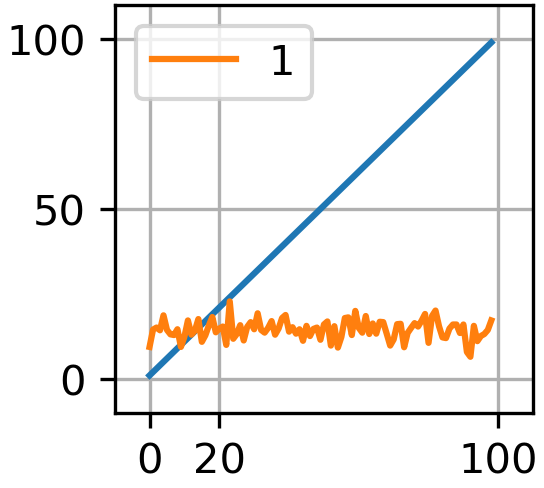
\includegraphics[width=0.25\linewidth]{pictures/out_pro 1}
	\hspace{0.01\linewidth}
	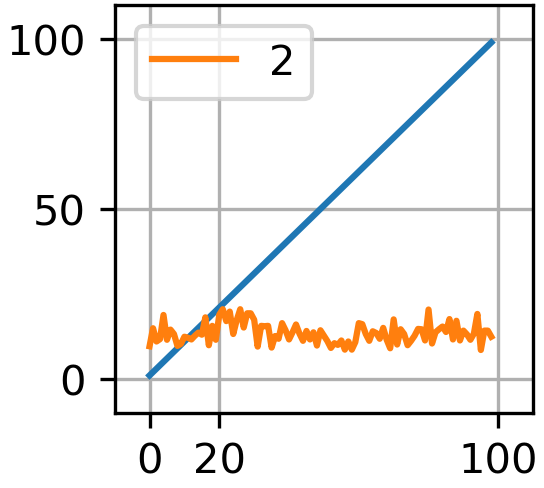
\includegraphics[width=0.25\linewidth]{pictures/out_pro 2}
	\hspace{0.01\linewidth}
	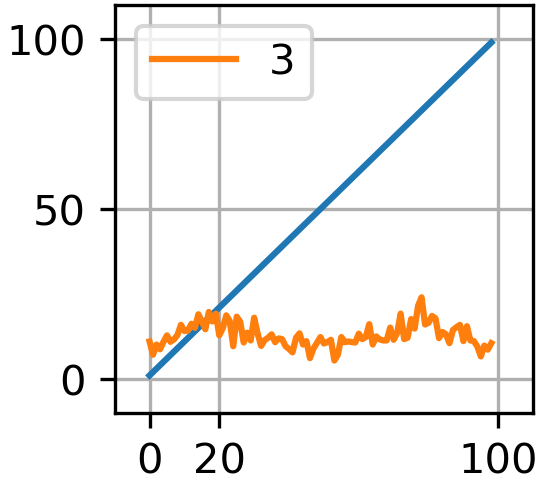
\includegraphics[width=0.25\linewidth]{pictures/out_pro 3}
	\\
	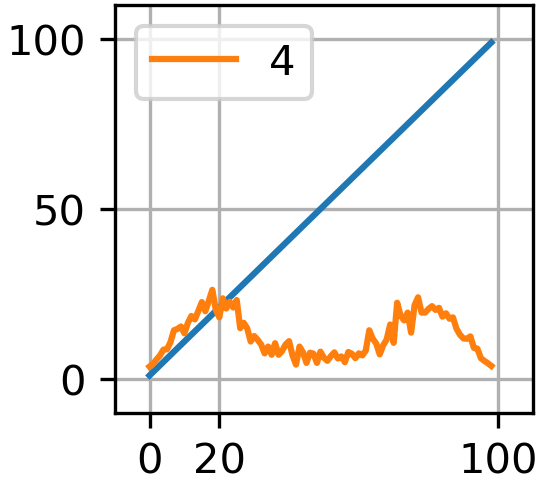
\includegraphics[width=0.25\linewidth]{pictures/out_pro 4}
	\hspace{0.01\linewidth}
	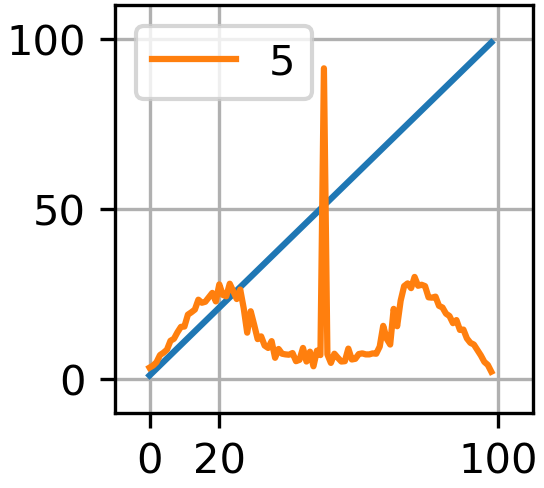
\includegraphics[width=0.25\linewidth]{pictures/out_pro 5}
	\hspace{0.01\linewidth}
	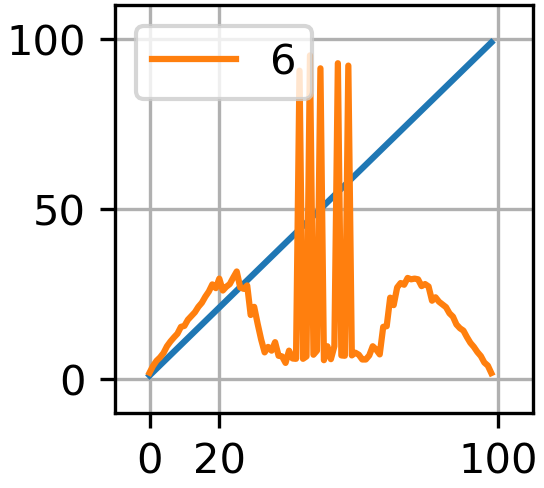
\includegraphics[width=0.25\linewidth]{pictures/out_pro 6}
	\\
	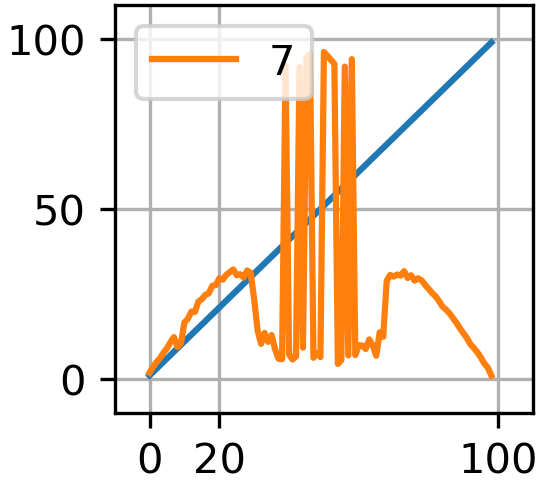
\includegraphics[width=0.25\linewidth]{pictures/out_pro 7}
	\hspace{0.01\linewidth}
	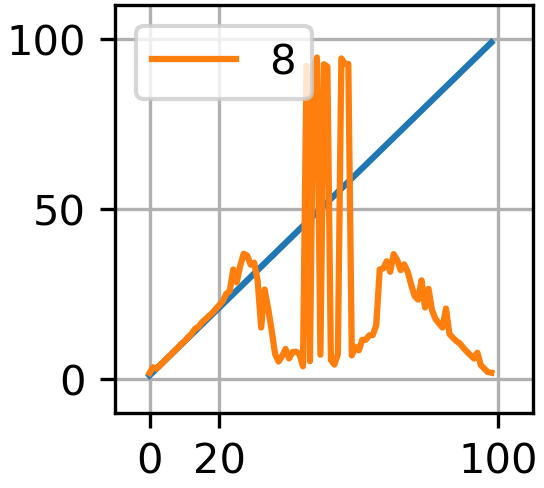
\includegraphics[width=0.25\linewidth]{pictures/out_pro 8}
	\hspace{0.01\linewidth}
	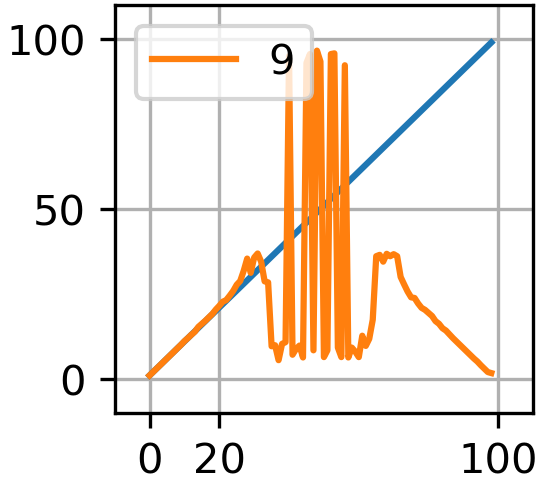
\includegraphics[width=0.25\linewidth]{pictures/out_pro 9}
	\\
	\caption{Синяя~--- заданный, зеленая~--- обнаруженный процент}
\end{figure}
Предварительно можно сказать, что наш алгоритм дает приемлемые результаты при выполнении следующих условий:

\medskip\noindent
\begin{enumerate}
	\item аномальные значения отличаются от нормальных значений на порядок и выше,
	\item процент аномальных значений не превышает 20\%.
\end{enumerate}

\section{Калибровочные границы}

После того, как в результате серии компьютерных экспериментов мы получили предварительные границы применимости нашего алгоритма, мы можем перейти собственно к процедуре вычисления калибровочных границ. Теперь это сделать очень легко: достаточно после вычисления номера \texttt{fold\_num} локтевой точки, которое мы провели на шаге 3.5 нашего алгоритма, принять в качестве допустимой границы отклонения величину \texttt{bound}:
\begin{verbatim}
bound = df_sorted['fluctation'].to_numpy()[fold_num]
\end{verbatim}
Например, если мы задаем следующие константы
\begin{verbatim}
	N = 1000
noise_mean = 0
noise_std = 0.1
\end{verbatim}
и следующие параметры генерации синтетических данных
\begin{verbatim}
out_pro  = 15
out_coef  = 6
\end{verbatim}
то коэффициент выраженности аномалии недостаточен для приемлемых результатов (см. раздел 4, шестую позицию рис. 3).  Действительно, в этом случае алгоритм возвращает в качестве прогнозируемого процента аномалий \texttt{out\_pro\_detected=21.6\%}, но это слишком сильно расходится с величиной параметра \texttt{out\_pro =15\%}, которую мы задали при генерации (см. первую позицию рис. 4). При этом возвращаемое алгоритмом значение допустимой границы отклонений, превышение которой означает аномалию, равно \texttt{bound=0.2264}, но ему нельзя доверять. Алгоритм отправил в аномальную зону слишком большой процент объектов, поэтому реальная калибровочная граница выше той, которую вернул алгоритм.

С другой стороны, если при тех же, что и выше, значениях констант мы выставим следующие параметры генерации
\begin{verbatim}
out_pro  = 15
out_coef  = 9
\end{verbatim}
то, согласно рассуждениям предыдущего раздела, алгоритм должен вернуть приемлемый результат (см. раздел 4, девятую позицию рис. 3).  И действительно, возвращаемый процент аномалий на этот раз не просто близок к заданному проценту аномалий, они буквально совпадают \texttt{out\_pro\_detected=15\%} (см. вторую позицию рис. 4) . Поэтому значение калибровочной границы, равное \texttt{bound=0.431}, вполне соответствует действительности.


\begin{figure}[!h]
	\centering
	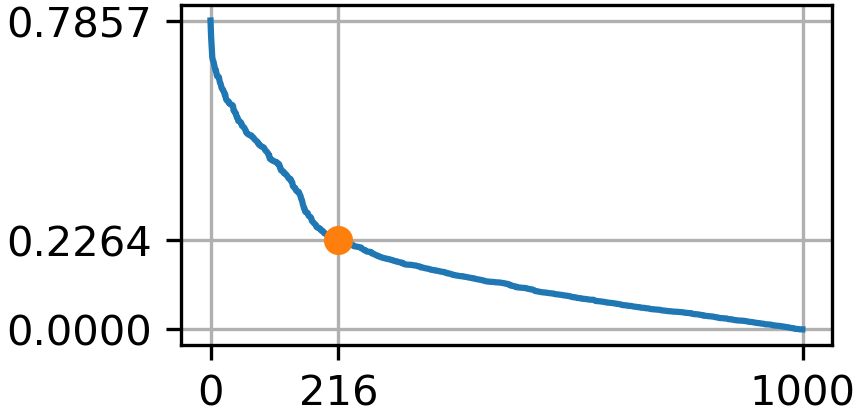
\includegraphics[width=0.4\linewidth]{pictures/bound 6}
	\hspace{0.05\linewidth}
	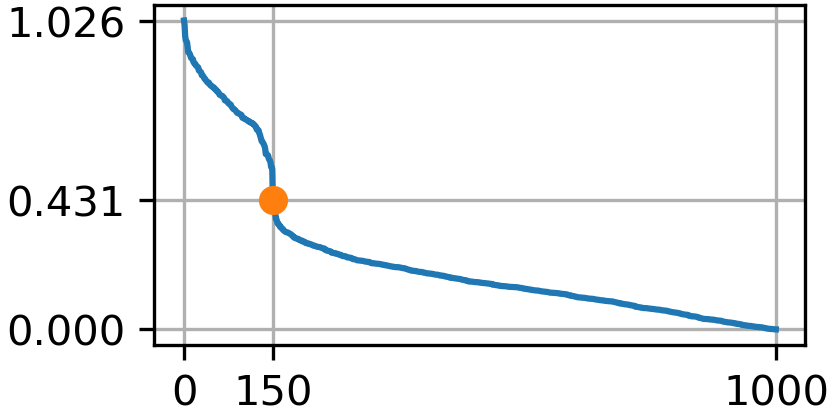
\includegraphics[width=0.4\linewidth]{pictures/bound 9}\\
	\caption{Примеры калибровочных границ}
\end{figure}

В качестве комментария к иллюстрациям рис. 4 добавим, что здесь мы визуализировали упорядоченные по убыванию отклонения из серии \texttt{df\_sorted['fluctation']} (синяя линия) и локтевую точку, которая была найдена при помощи функции \texttt{fold\_point} (желтая точка).


\section{Выводы и рекомендации}

Предложенный нами алгоритм не только детектирует аномальные значения, но и самостоятельно устанавливает калибровочные границы, то есть величины отклонений, превышение которых означает аномалию. Это бывает очень важно, особенно в ситуациях, когда и сама измеряемая величина, и ее вариация изменяются с течением времени, например, при измерении биржевых показателей.

Вместе с тем, следует отметить, что наш алгоритм имеет ряд существенных ограничений. Прежде всего, это отмеченные нами выше ограничения на выраженность аномалий и их долю в общем числе наблюдений (см. раздел 4). Однако гораздо более существенным является логическое ограничение, состоящее в том, что для корректного применения нашего алгоритма необходимо заранее знать хотя бы приблизительно то,  насколько выражены аномалии в наборе данных и каков их процент. 

Если, исходя из каких-либо внешних по отношению к данным соображений, мы заранее знаем, что выраженность аномалий составляет примерно порядок или выше, а их объем не превышает 20\% от объема выборки, мы можем быть уверены, что алгоритм вернет приемлемый результат. Для такого знания нужны какие-то (в разных ситуациях — разные) представления о предметной области, из которой получены данные, что противоречит «чистому» анализу, который ведется вслепую, без апелляции к предметной области.
Но практический анализ данных без знания предметной области, видимо, не возможен.



\section{Литература}

\begin{enumerate}
	\item Хейдт М. Изучаем Pandas / М. Хейдт;  — Москва: ДМК Пресс, 2018. — 438 с. 
	\item Бурков А. Машинное обучение без лишних слов / А. Бурков;  — СПб: Питер, 2020. — 192 с.
	\item Вьюгин, В. В. Математические основы теории машинного обучения и прогнозирования / В. В. Вьюгин; — М.: МЦИМО. — 2013. — 387~с. 
	\item Бринк Х. Машинное обучение / Х. Бринк, Дж. Ричардс, М. Феверолф  — СПб.: Питер, 2017. — 336 с.
	\item Мосин, В. Г. Линеаризация целевой функции в регрессионных задачах методом сингулярных разложений / В. Г. Мосин // Математическое моделирование : Тезисы II Международной конференции, Москва, 21–22 июля 2021 года. – Москва: Издательство Перо, 2021. – С. 66--67.
\end{enumerate}



\end{document}
